\documentclass[a4paper,12pt]{article}

\usepackage{other/lab_preamble}

\numberwithin{equation}{section}

\begin{document}

\LabTitle{2.2.1}{Исследование взаимной диффузии газов}

\tableofcontents
\listoffigures
\listoftables

\newpage

\textbf{Цель работы}:
\begin{enumerate}
  \item регистрация зависимости концентрации гелия в воздухе от времени с помощью датчиков теплопроводности при разных начальных давлениях смеси газов
  \item определение коэффициента диффузии по результатам измерений.
\end{enumerate}

\textbf{Приборы}:
\begin{enumerate}
  \item измерительная установка
  \item форвакуумный насос
  \item баллон с газом (гелием)
  \item манометр
  \item источник питания
  \item магазин сопротивлений
  \item гальванометр
  \item секундомер
\end{enumerate}

\section{Краткая Теория.}
\textit{Диффузией}  называют самопроизвольное взаимное проникновение веществ друг в друга происходящее вследствие хаотичного теплового движения молекул. При перемешивании молекул разного сорта говорят о взаимной (или концентрационной) диффузии. В системе, состоящей из двух компонентов a и b (бинарная смесь), плотности потоков частиц в результате взаимной диффузии определяются законом Фика:
\begin{equation}
  j_a = -D \frac{\partial n_a}{\partial x}, \quad j_b = -D \frac{\partial n_b}{\partial x}
\end{equation}

\begin{description}
  \item[D] - \textit{коэффициент взаимной диффузии компонентов}
  \item[$j_{a, b}$] - плотности потока, частиц, соответствующего сорта
  \item[$n_{a, b}$] - концентрации газов
\end{description}

В данной работе исследуется взаимная диффузия гелия и воздуха. Давление и температура в системе предполагаются неизменными.\\
\[n_{He} \ll n_{air}\]
Поэтому изменение концентрации воздуха в результате взаимной диффузии будет незначительной. В дальнейшем мы будем описывать только диффузию примеси
гелия на стационарном фоне воздуха и под n будем иметь в виду концентрацию $n_{He}$. \par

\begin{figure}[H]
  \centering
  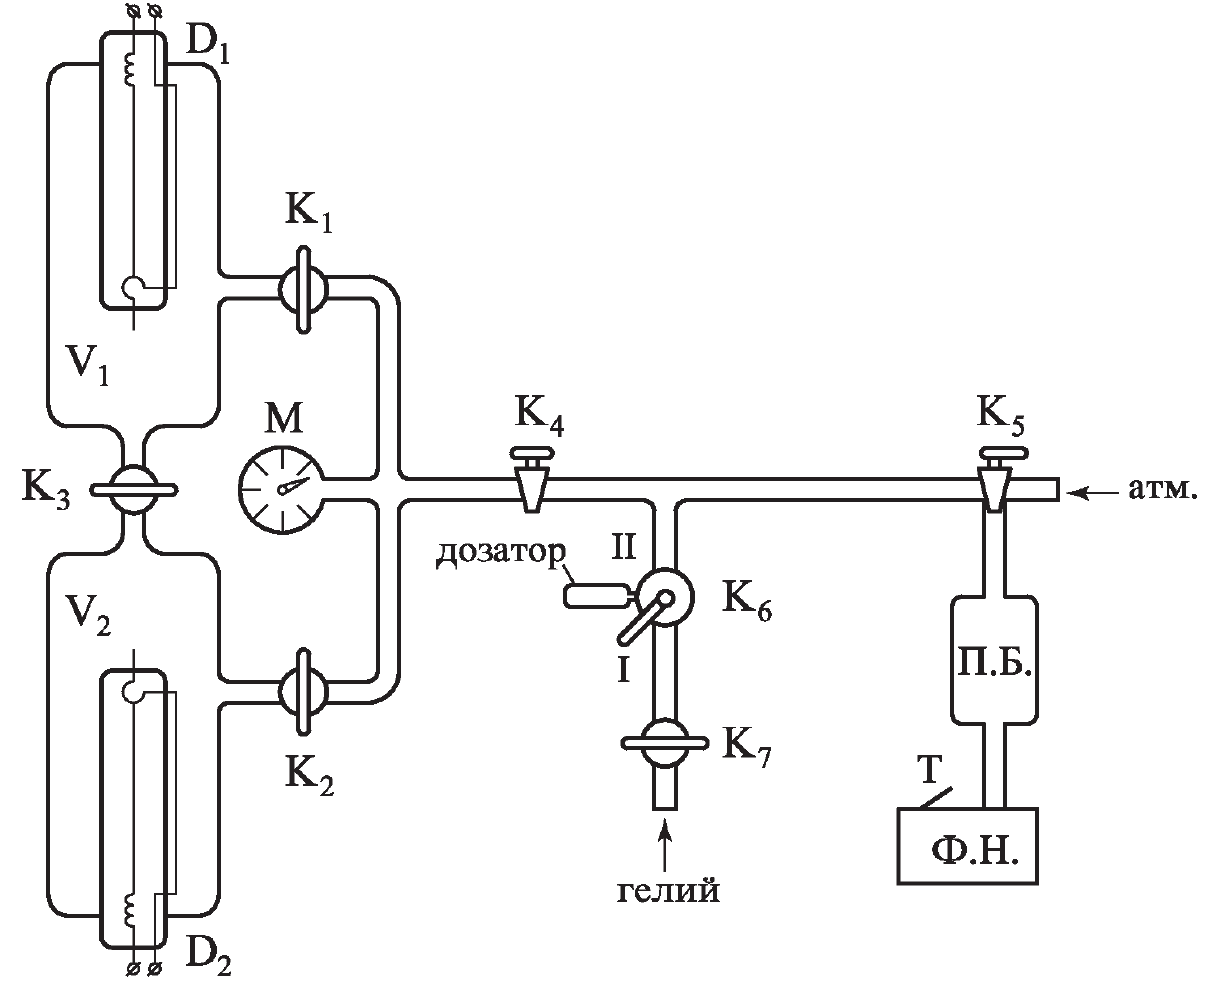
\includegraphics[scale=0.5]{data/fig1.png}
  \caption[Установка.]{Установка для исследования взаимной диффузии газов.}
  \label{fig:1}
\end{figure}

В работе используется установка, изображённая на рис. \ref{fig:1}. \\
Два сосуда с объёмами $V_1$ и $V_2$ соединены трубкой длины l и сечения S. \\
Сосуды заполнены смесью двух газов при одинаковом давлении, но с различной концентрацией компонентов. \\
Вследствие взаимной диффузии концентрации в обоих сосудах с течением времени выравниваются. \par
Рассмотрим процесс выравнивания концентрации. В трубке устанавливается стационарный поток частиц:
\begin{equation}
  J = -DS \partderiv{n}{x} = -DS \frac{n_1 - n_2}{l}
\end{equation}

Пусть $\D{n_1}$ и $\D{n_2}$ -изменения концентрации в $V_1$ и $V_2$.
\begin{equation}
  V_1 \D{n_1} = -V_2 \D{n_2} = J \D{t} = -DS \frac{n_1 - n_2}{l} \D{t} \quad \implies
\end{equation}
\begin{equation}
  V_1 \deriv{n_1}{t} = -V_2 \deriv{n_2}{t} = -DS \frac{n_1 - n_2}{l} \quad \implies
\end{equation}
\begin{equation}
  \deriv{n_1}{t} - \deriv{n_2}{t} = 
  -DS \frac{n_1 - n_2}{l} \left(\frac{1}{V_1} + \frac{1}{V_1}\right) \quad \implies
\end{equation}

Пусть \[ \D{n} \triangleq n_1 - n_2 \] \par Тогда:
\begin{equation}
  \D{n} = n_0 e^{-t / \tau} \label{eq:delta_n}
\end{equation}
\begin{description}
  \item[$n_0$] - разность концентраций примеси в начальный момент времени
\end{description}

\begin{equation}
  \tau = \frac{V_1 V_2}{V_1 + V_2} \frac{l}{SD}
  \label{eq:1.7}
\end{equation}

Для проверки применимости квазистационарного приближения необходимо убедиться, что время $\tau$ много больше характерного времени диффузии:
\[ t_{\text{дифф}} \approx \frac{l^2}{D} \ll \tau \]

\subsection{Методика измерений.}

Для измерения концентраций в данной установке применяются датчики теплопроводности
$D_1$ и $D_2$ \seefigref{fig:1}. \\
Тонкая проволочка радиуса $r_\text{пр}$, протянутая вдоль оси стеклянного цилиндра радиуса $R_\text{ц}$, нагревается током.

\begin{equation}
  Q = k \frac{2\pi L}{\ln{R_\text{ц} / r_\text{пр}}} (T_1 - T_2)
\end{equation}
\begin{description}
  \item[k] - теплопроводность
  \item[$r_\text{пр}$] - радиус проволки
  \item[$R_\text{ц}$] - радиус цилиндра
  \item[L] - длина проволки
  \item[$T_1,\ T_2$] - температура проволки и стенки сосуда
\end{description}

Для измерения разности концентраций газов используется мостовая схема \seefigref{pic:2}.
Мост балансируется при заполнении сосудов одной и той же смесью.

При малых изменениях концентрации можно считать, что \[ V \thicksim k \thicksim n \]
Тогда: 
\begin{equation}
  V = V_0 e^{-t/\tau} \label{eq:V}
\end{equation}

\subsection{Экспериментальная установка.}


\section{Ход работы}
\begin{enumerate}
  \item Ознакомимся с установкой.
  
  \item Включим питание электрической схемы установки рубильником B. \\
  Откроем краны $K_1, K_2, K_3$.
  
  \item Очистим установку от газов. \\ Для этого:
  \begin{enumerate}
    \item Изолируем систему от атм. давления.
    \item Откроем кран $K_4$.
    \item Включим насос.
    \item Соединим насос с установкой краном $K_5$.
    \item Откачаем установку до минимального значения на гальванометре. \\
    (это занимает 1-5 мин.)
    \item Отключим насос.
    \item Перекроем $K_4$.
    \item Соединим насос с атмосферой краном $K_5$.
  \end{enumerate}

  \item Запустим в установку воздух до рабочего давления $P_{\text{раб}}$ \\
  (вначале $P_{\text{раб}} \approx 40\ \torr$).\\
  Конкретный метод зависит от установки. \\
  Сбалансируем мост. Для этого добьемся примерно нулевого значения на гальванометре, поворачивая ручки "грубо" и "точно". Диапазон измерений гальванометра переведем на 10 мкА.

  \item Заполним установку рабочей смесью.
  В сосуде $V_2$ должен быть воздух, а в сосуде $V_1$ — смесь воздуха с гелием.
  Для этого:
  \begin{enumerate}
    \item Откачаем установку.
    \item Закроем $K_2$ и $K_3$ (Изолируем $V_2$).
    \item Убедимся: $K_5$ закрыт, $K_1$ и $K_4$ открыты.
    \item Заполним $V_1$ гелием до $P_{He} = x \cdot P_{\text{раб}}$ 
    ($x$ зависит от установки). \\
    Для этого будем постепенно запускать гелий в промежуток между $K_6$ и $K_7$ и из него в установку.
    \item Закроем $K_1$ (Изолируем $V_1$).
    \item Прочистим трубы от гелия. Для этого откачаем его насосом.
    \item Откроем $K_2$ (Соединим $V_2$).
    \item Заполним $V_2$ воздухом до давления $P_{air} = y \cdot P_{\text{раб}}$
    ($y$ зависит от установки). \\
    \item Закроем $K_4$.
    \item Уравняем давление в объёмах $V_1$ и $V_2$. \\
    Для этого откроем $K_1$ и подождем 30-60 с.
    \item Закроем $K_1$ и $K_2$.
  \end{enumerate}

  \item Приступим к измерениям зависимости $n_{He}$ от времени.
  Для этого запустим утилиту на компьютере и откроем $K_3$.

  \item Проделаем пункты 3-6 при 5-6 значениях $P_{\text{раб}}$ в интервале 40-400 торр.
  
  \item Убедимся, что процесс диффузии подчиняется закону \eqref{eq:delta_n}.
  Для этого построим графики $(t, \ln{(n(t))})$ и по наплонам прямых расчитать коэффициенты взаимной диффузии.

  Данные представлены в виде зависимости V(t), где V - показания гальвонометра. \\
  Справедлива формула \ref{eq:V}, поэтому достаточно воспользоватся зависимостью V(t). \\

  \begin{figure} [H]
    \center
    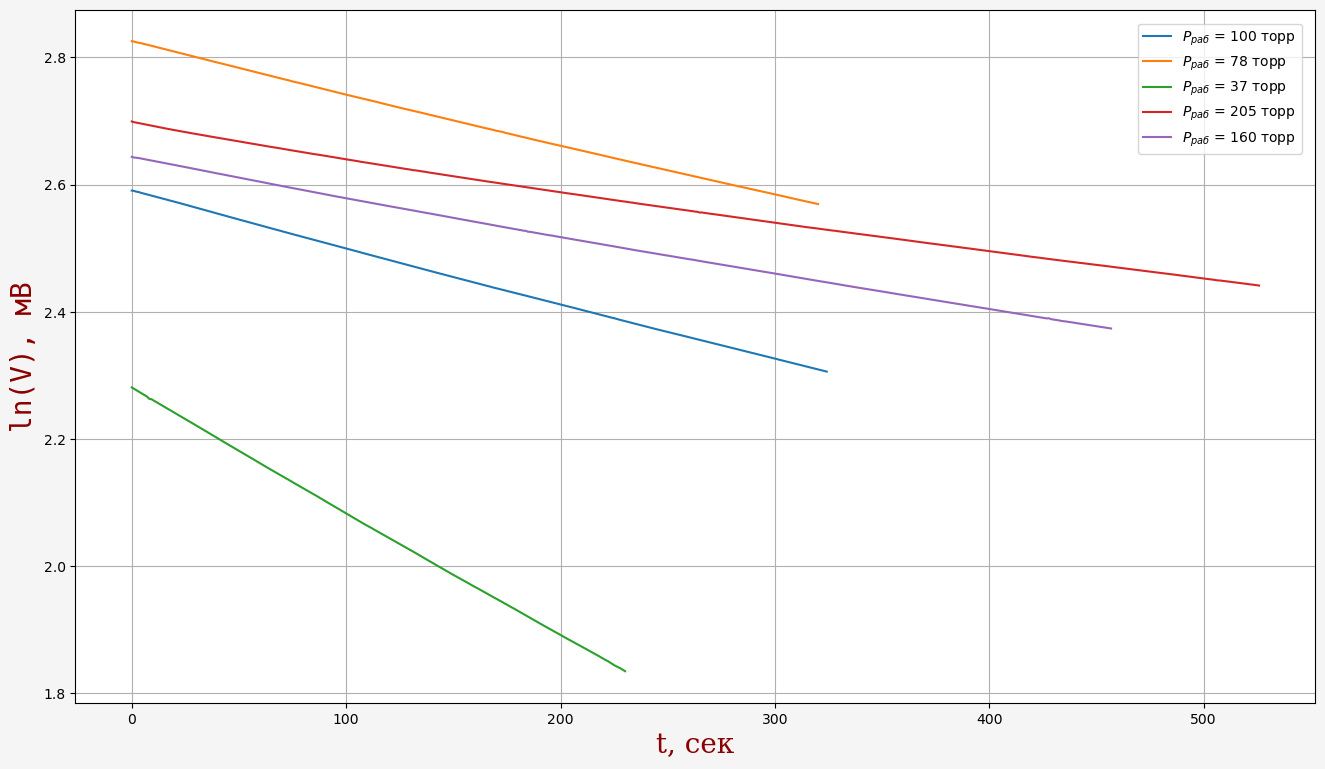
\includegraphics[scale=0.5]{./data/graph1.png}
    \label{fig:graph:(t, ln(V))}
  \end{figure}

  \item Построим график (D, 1/$P_{\text{раб}}$). График должен иметь вид прямой линии. \\
  По формуле \eqref{eq:V} Получим, что 

  \begin{equation}
    slope = \frac{1}{\tau} \implies \eqref{eq:1.7} \implies D =
     - slope \cdot \frac{V_1 V_2}{V_1 + V_2} \cdot \frac{L}{S}
    \label{eq:2.1}
  \end{equation}

  \begin{figure} [H]
    \center
    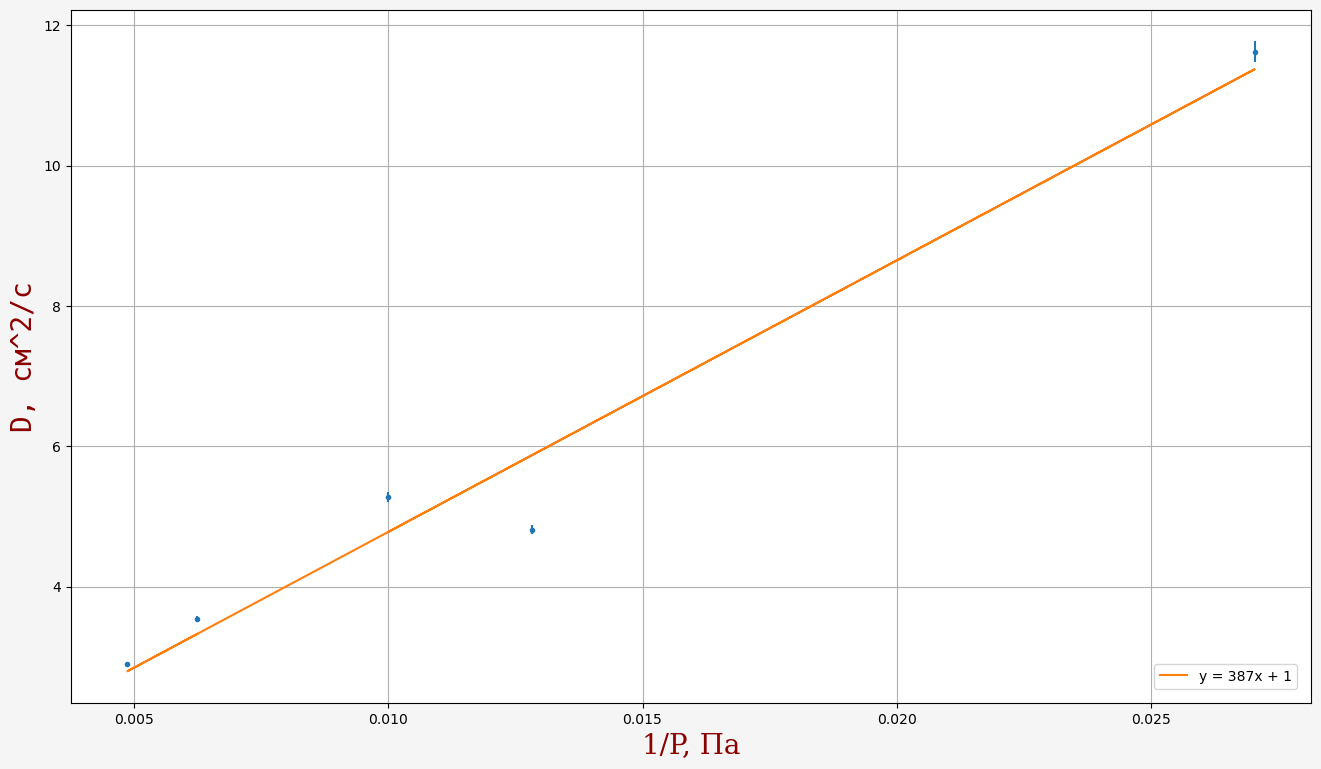
\includegraphics[scale=0.5]{./data/graph2.png}
    \label{fig:graph:D(1/P)}
  \end{figure}

  \begin{table} [H]
    \center
    \begin{tabular}{|l|l|l|l|}
    \hline
    $P,\ \Pa$&$D,\ \cm^2/\sec$&$slope,\ \Pa \cdot \cm^2/\sec$\\
    \hline
    37&$11.63 \pm 0.15$&$(-19377 \pm 13) \cdot 10^{-6}$\\
    78 &$4.81 \pm 0.06$&$(-8017  \pm  9) \cdot 10^{-6}$\\
    100&$5.28 \pm 0.07$&$(-8799  \pm  8) \cdot 10^{-6}$\\
    160&$3.54 \pm 0.05$&$(-5893  \pm  9) \cdot 10^{-6}$\\
    205&$2.89 \pm 0.04$&$(-4816  \pm 11) \cdot 10^{-6}$\\
    \hline
    \end{tabular}
    \caption{Зависимость коэфф-ов взаимной диффузии воздуха и гелия при давлении P \eqref{eq:2.1}. \label{table:P-D-slope}}
  \end{table}

  Рассчитаем величину коэффициента диффузии при атмосферном давлении. \\

  По мнк получим коэффициенты прямой $y = \alpha x + \beta$:
  \[ \alpha = (387 \pm 40)\ \Pa \cdot \frac{\cm^2}{\sec} \]
  \[ \beta = (0.9 \pm 0.6)\ \frac{\cm^2}{\sec} \]

  \[ D(P_\text{атм}) \approx \beta \]

  \item Оценим по полученным результатам длину свободного пробега и размер молекулы.

  По закону Менделеева-Клапейрона:
  \begin{equation}
    PV = \nu RT \implies n = \frac{P N_A}{RT}
  \end{equation}

  Найдем концентрацию воздуха:
  \begin{equation}
    n_\text{в} = \frac{P_\text{раб} V_1}{RT} \approx P_\text{раб} \cdot 
  \end{equation}

  


\end{enumerate}

\subsection{Вывод.}
В данной рабобте мы измерили зависимость изменения концентрации гелия в воздухе от времени при различных давлениях (\figref{fig:graph:(t, ln(V))}).\\
Определили коэффициенты взаимной диффузии (т. \ref{table:P-D-slope})  и построили график D(1/P) \seefigref{fig:graph:D(1/P)}.


\end{document}